\documentclass[12pt]{book}

\usepackage[T1]{fontenc}
\usepackage[right=0.5in,left=1in,top=1in,bottom=1in]{geometry}
\usepackage{graphicx}
\usepackage{wrapfig}
\usepackage{hyperref}
\usepackage{tabularx}
\usepackage{array}
\usepackage{amsmath}
\usepackage{amssymb}
\usepackage{fancyhdr}
\usepackage{lastpage}
\usepackage{titlesec}
\usepackage{xcolor}
\usepackage{fontawesome5}


\titlespacing*{\section}{0pt}{1.6ex}{0.2\baselineskip}
\titlespacing*{\subsection}{0pt}{0.1\baselineskip}{0.2\baselineskip}


\begin{document}
\pagestyle{fancy}
\thispagestyle{empty}
\fancyhead[L]{Miraj Samarakkody}
\fancyhead[R]{Curriculum Vitae}
\fancyfoot[C]{Page \thepage\ of \pageref{LastPage}}
%\begin{minipage}{0.25\textwidth}
%	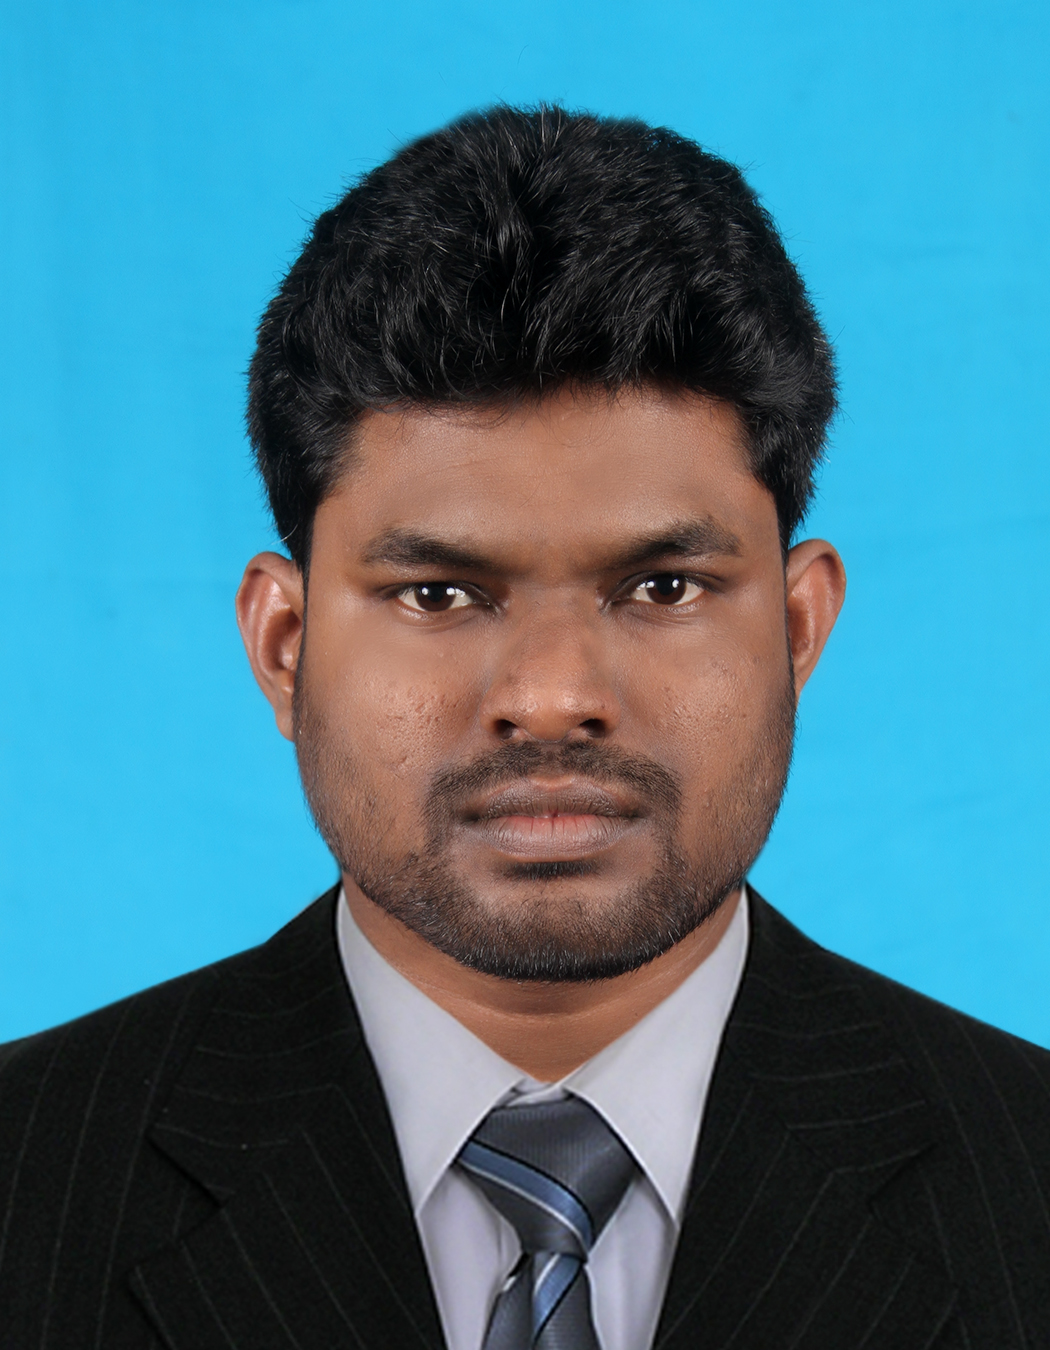
\includegraphics{Figures/image.jpg}
%\end{minipage}%
%\begin{minipage}{0.75\textwidth}
\begin{center}
\textbf{\Huge{Miraj Chamara Samarakkody}}\\
\end{center}
%\vspace{0.1in}

``Dedicated to advancing research and academic excellence in differential geometry, committed to contributing to the growth of both the institute and society with my full potential."

\begin{center}
\textbf{S Rajakaruna Samarakkodige Miraj Chamara Samarakkody}
\end{center}
  \faPhone\ \href{tel:+17696016290}{+1 (769) 601 6290} \hfill \faEnvelope\  \href{mailto:miraj.samarakkody@gmail.com}{miraj.samarakkody@gmail.com} \hfill \faGlobe\ \href{https://mirajcs.github.io/}{mirajcs.github.io}\\

\section*{Research Interest} \rule{\textwidth}{1pt}\\

Minimal surfaces, generalized elastic curves, and applications of differential geometry in mathematical physics, biology, and data science.\\

\section*{Professional Experiences} \rule{\textwidth}{1pt}\\

\begin{itemize}

\item \textbf{Assistant Professor} \hfill \textbf{Spring 2025 - Present}\\
Department of Mathematics and Computer Science, Tougaloo College, MS.

	\item \textbf{Graduate Part-Time Instructor} \hfill \textbf{Fall 2024}\\
Department of Mathematics \& Statistics, Texas Tech University, TX.



\item \textbf{Research Assistant} \hfill \textbf{Spring 2022 - Summer 2024} \\
Mentors: Dr. Hung Tran and Dr. \'Alvaro P\'ampano.\\
Department of Mathematics \& Statistics, Texas Tech University.

\item \textbf{Graduate Teaching Assistant} \hfill \textbf{Fall, 2021}\\
%Calculus II with Applications (MATH 1452)\\
Department of Mathematics \& Statistics, Texas Tech University.

%\item \textbf{Lecturer (Probationary)} \hfill \textbf{November, 2019 - July, 2021}\\
%Faculty of Engineering, University of Moratuwa, Sri Lanka.

%\item \textbf{Visiting Lecturer} \hfill \textbf{January, 2021 - June, 2021}\\
%Faculty of Humanities and Sciences, Sri Lanka Institute of Information Technology, Sri Lanka.

%\item \textbf{Visiting Lecturer} \hfill \textbf{February, 2021 - May, 2021}\\
%Faculty of Engineering, University of Sri Jayewardenepura, Sri Lanka.

%\item \textbf{Visiting Lecturer} \hfill \textbf{January, 2019 - July, 2019}\\
%General Sir John Kotelawala Defence University, Ratmalana, Sri Lanka.

%\item \textbf{Temporary Assistant Lecturer} \hfill \textbf{December, 2018 - February, 2019}\\
%Faculty of Science, University of Peradeniya, Sri Lanka.

%\item \textbf{Temporary Tutor} \hfill \textbf{January, 2018 - December, 2018}\\
%Faculty of Science, University of Peradeniya, Sri Lanka.
\end{itemize}

\section*{Short Visits}  \rule{\textwidth}{1pt}\\

\begin{itemize}
	\item \textbf{Research Mentor} \hfill \textbf{Summer 2025}\\
Virtual Math Circle, Department of Mathematics, Louisiana State University.
\end{itemize}


\section*{Education} \rule{\textwidth}{1pt}\\

\noindent \textbf{Texas Tech University, TX.} \hfill \textbf{Fall 2021 - Spring 2024}\\
Ph.D. in Mathematics, May, 2025. \\
%Dissertation: ``\textit{\textbf{On Some Variational Problems in Curves and Surfaces}}''\\
Advisors:  \href{https://www.myweb.ttu.edu/tra97432/}{Dr. Hung Tran} (Chair), \href{https://www.math.ttu.edu/~apampano/}{Dr. \'Alvaro P\'ampano} (Co-chair).\\

\noindent \textbf{University of Peradeniya, Sri Lanka.} \hfill \textbf{2014-2018}\\
B.Sc. (Honors) Special in Mathematics. \\
%Project: ``\textit{\textbf{Geometric Behavior of a Certain Class of Quotients of Finite Blaschke Products.}}''\\
Advisor: Dr. Shelton Perera. 

\section*{Languages}
\rule{\textwidth}{1pt}
\begin{itemize}
	\item \textbf{English} - Excellent Proficiency.
	\item \textbf{Sinhala} - Native Proficiency. 
\end{itemize}


\section*{Technical Skills}
\rule{\textwidth}{1pt}\\

\LaTeX, Julia, Python, Mathematica, Matlab, Lingo, Maple, Microsoft Office, Adobe Illustrator and Adobe Premier Pro. \\


\section*{Teaching}
\rule{\textwidth}{1pt}\\
%\subsection*{Research}

%\begin{itemize}
%	\item \textbf{Research Mentor} \hfill \textbf{Summer, 2025}\\
%	\textbf{Topics:}
%	\begin{itemize}
%%		\item Hyperbolic Functions and Their Applications in Engineering and Architecture. 
%	\end{itemize}
%	Virtual Math Circle, Department of Mathematics, Louisiana State University.

%	\item \textbf{Research Assistant} \hfill \textbf{Spring, 2022-Summer, 2024}\\
 %Advisors:  Dr. Hung Tran and Dr. \'Alvaro P\'ampano.  \\
%Research focused on Morse index of minimal surfaces and generalized elastic curves. \\
%Department of Mathematics \& Statistics, Texas Tech University. 

%\end{itemize}



%\subsection*{Teaching}
\subsection*{Tougaloo College}
	\vspace{1em}

\begin{itemize}
	\item \textbf{MAT221 - Calculus I}; Fall 2025
	\item \textbf{MAT222 - Calculus II}; Spring 2025
	\item \textbf{MAT316 - Differential Equations}; Fall 2025
	\item \textbf{MAT326 - Introduction to Probability}; Fall 2025
	\item \textbf{MAT414 - Modern Algebra}; Spring 2025
	\item \textbf{MAT426 - Advanced Calculus}; Spring 2025, Fall 2025
	\item \textbf{MAT434 - Theory of Mathematical Statistics}; Spring 2025
	%\item 
%Department of Mathematics and Computer Science, Tougaloo College.
%	\item \textbf{Graduate Part-Time Instructor (Instructor of Records)} \hfill \textbf{Fall, 2024}\\
%Calculus II with Applications (MATH 1452-122)\\
%Department of Mathematics \& Statistics, Texas Tech University.
%\item \textbf{Graduate Teaching Assistant} \hfill \textbf{Fall, 2021}\\
%Calculus II with Applications (MATH 1452)\\
%Department of Mathematics \& Statistics, Texas Tech University.
%\item \textbf{Lecturer } \hfill \textbf{Semester II, 2021}\\
%Neural Networks \& Fuzzy Logic (MA4144)\\
%Faculty of Engineering, University of Moratuwa, Sri Lanka.
%\item  \textbf{Lecturer} \hfill \textbf{Semester II, 2021}\\
%Ordinary Differential Equations (MA3013)\\
%History of Mathematics (MA3022)\\
%Faculty of Humanities and Sciences, Sri Lanka Institute of Information Technology, Sri Lanka.

%\item \textbf{Lecturer} \hfill \textbf{Semester II, 2021}\\
%Discrete Mathematics (IS 3202)\\
%Faculty of Engineering, University of Sri Jayewardenepura, Sri Lanka.

%\item  \textbf{Lecturer }\hfill\textbf{ Semester I, 2020}\\
%Calculus (MA2024)\\
%Faculty of Engineering, University of Moratuwa, Sri Lanka. 

%\item  \textbf{Lecturer}\hfill  \textbf{Semester II, 2019}\\
%Mathematics for IT\\
%General Sir John Kotelawala Defence University, Ratmalana, Sri Lanka.

%\item \textbf{Teaching Assistant} \hfill \textbf{Semester II, 2018}\\
%Group Theory (MAT3013), Complex Analysis I (MAT3122)\\
%University of Peradeniya, Sri Lanka.

%\item \textbf{Teaching Assistant} \hfill \textbf{Semester I, 2018}\\
%Real Analysis III (MAT3023), Functional Analysis (MAT4033)\\
%University of Peradeniya, Sri Lanka. 
\end{itemize}

\subsection*{Texas Tech University}
\begin{itemize}
	\item \textbf{MATH 1452 - Calculus II with Applications}; Fall 2024
\end{itemize}



\section*{Grants} \rule{\textwidth}{1pt}

\begin{itemize}
	\item \textbf{PI}, SCALE Program (Partenership with Purdue University), $\$73,094.77$.\\
	\textbf{Project:} Microelectronic Workforce Development Project for Radiation-Hardening.
\end{itemize}

\section*{Fellowships}
\rule{\textwidth}{1pt}
\begin{itemize}
	\item \textbf{Dr. Shelby Hildebrand Graduate Math Fellowship}  - Texas Tech University.   \hfill 2023-2024\\
	Amount: \$10,000
	\item \textbf{AT \& T Graduate Fellowship} - Texas Tech University \hfill 2021-2025\\
	Amount: \$16,000
\end{itemize}


























\section*{Awards and Honors}
\rule{\textwidth}{1pt}

\begin{itemize}
	\item \textbf{Create Possible Scholarship} - Texas Tech University. \hfill 2022
	\item \textbf{University Prize for Academic Excellence} - University of Peradeniya \hfill 2018
	\item \textbf{Peradeniya University Alumni Australia Victoria Chapter Scholarship for Academic Excellence in Mathematics} \hfill 2015
\end{itemize}

%\newpage


\section*{Presentations}
\rule{\textwidth}{1pt}\\
\subsection*{Conference Talks}
%\vspace{0.1in}
\begin{itemize}
	\item ``\textit{\textbf{Closed $p-$Elastic Curves in 2-Space Forms},}'' AMS Sectional Meeting (Meeting No: 1198), University of Texas, San Antonio, September 14-15, 2024.
	\item ``\textit{\textbf{Closed p-Elastic Curves in Spheres of Lorentz-Minkowski Space.}}'', Texas Analysis and Mathematical Physics Symposium, Texas A\&M University, February 10, 2024.
	\item ``\textit{\textbf{Geometric Behavior of a Certain Class of Quotients of Finite Blaschke Products}}'', ICMME, Post Graduate Institute of Science, University of Peradeniya, March, 2019
\end{itemize}

\subsection*{Posters}
\begin{itemize}
	\item ``\textit{\textbf{Closed $p-$Elastic Curves in 2-Space Forms},}'' Texas Geometry and Topology Conference (68th Meeting),  Texas A\&M University, College  Station, November 8-10, 2024.
\end{itemize}

\subsection*{Seminars}
\begin{itemize}
	\item ``\textit{\textbf{On Some Variational Problems in Curves and Surfaces}}''- Probability, Differential Geometry and Mathematical Physics Seminar, Texas Tech University (January $21^{st}$, 2025).
	\item ``\textit{\textbf{On Some Variational Problems in Differential Geometry}}''- Probability, Differential Geometry and Mathematical Physics Seminar, Texas Tech University (November $01^{st}$, 2023).

\item ``\textit{\textbf{Minimal Surfaces}}''-Probability, Differential Geometry and Mathematical Physics Seminar, Texas Tech University (November $02^{nd}$, 2022)

\end{itemize}


%\subsection*{Outreach Programs}
%\begin{itemize}
%	\item ``\textit{\textbf{Brainstorming Math Questions IV}}'' Math Circle, Department of Mathematics \& Statistics, Texas Tech University. (March $28^{th}$, 2024).
%	\item ``\textit{\textbf{Brainstorming Math Questions III}}'' Math Circle, Department of Mathematics \& Statistics, Texas Tech University. (March $21^{th}$, 2024).
%\item ``\textit{\textbf{Brainstorming Math Questions II}}'' Math Circle, Department of Mathematics \& Statistics, Texas Tech University. (November $29^{th}$, 2023).
%\item ``\textit{\textbf{Brainstorming Math Questions I}}'' Math Circle, Department of Mathematics \& Statistics, Texas Tech University. (November $8^{th}$, 2023). 
%\item ``\textit{\textbf{Some Geometric Problems}}'' Math Circle, Department of Mathematics \& Statistics, Texas Tech University. (October $11^{th}$, 2023)
%\item ``\textit{\textbf{Minimal Surfaces and Generalized Elastic Curves}}'' - 3MT, Texas Tech University (October $6^{th}$, 2023).

%\end{itemize}



\section*{Publications}
\rule{\textwidth}{1pt}
\begin{itemize}
	\item A. P\'ampano, \underline{M. Samarakkody}, H. Tran, ``\textit{\textbf{Closed $p-$Elastic Curves in Spheres of $\mathbb{L}^{3}$,}}'' JMAA, 542(2):129147, 2025. 
 \item \underline{S.R.S.M.C. Samarakkody}, P.G.R.S. Ranasinghe, A.A.S. Perera, ``\textit{\textbf{Geometric Behavior of a Certain Class of Quotients of Finite Blaschke Products}},'' ICMME, Post Graduate Institute of Science, University of Peradeniya, Vol. 1. (2019).
\end{itemize}





 
 \section*{Leadership and Community Involvement}
\rule{\textwidth}{1pt}
\begin{itemize}
	\item ``\textbf{Summer Chess Camp 2024},'' \textit{Counselor}, Texas Tech University. 
	\item ``\textbf{Art \& Humanities Conference 2023},'' \textit{Judge}, Texas Tech University.  
	\item ``\textbf{Math Circle 2023-2024},''\textit{Mentor}, Department of Mathematics \& Statistics, Texas Tech University. 
	%\item \textit{Lubbock Library Volunteer}, Lubbock.
\end{itemize}





\section*{Memberships in Professional Societies}
 \rule{\textwidth}{1pt}
 \begin{itemize}
 	\item Member of \textbf{American Mathematical Society}. \hfill  2021-2025
	\item Member of \textbf{SIAM TTU Chapter.} \hfill 2021-2025
 \end{itemize}





\end{document}
